\chapter{Анализ графов спутников полученных при помощи polaris 2.0}

Для оценки влияния космической погоды на бортовые системы и целевую аппаратуру
малых космических аппаратов (МКА) в этой главе будет проведен комплексный анализ
зависимости параметров телеметрии \cite{green_2017_impact}
\cite{schlag_2018_numerical} \cite{boumghar_2018_enhanced}, индексов солнечной
активности и геомагнитных индексов. В основе исследования лежит применение
модели машинного обучения Polaris ML. Результаты работы модели будут
представлены в виде двухмерного графа связности, отражающего выявленные
взаимосвязи между исследуемыми параметрами.

Для расчета и анализа графа связности будет использована обширная база данных
телеметрии сети наземных станций SatNOGS. Параметры солнечной активности будут
извлечены из следующих основных источников:

\begin{itemize}
	\item Центр прогнозирования космической погоды (Space Weather Prediction Center, SWPC/SWO) \cite{swpc_noaa_data_souce};
	\item Центр наблюдения и анализа данных о влиянии Солнца в Брюсселе (Solar Influences Data Analysis Center, S.I.D.C.) \cite{silso_snd_data_source};
	\item Канадская радиоастрофизическая обсерватория в Пентиктоне \cite{swgc_flux_data_source}.
\end{itemize}

Далее представлена таблица \ref{tab:detailed_solar_geo_params} с основными анализируемыми параметрами солнечной активности

\begin{longtable}{|l|p{12cm}|}
	\caption{Подробное описание параметров солнечной и геомагнитной активности}
	\label{tab:detailed_solar_geo_params}                                                                                                                                                                                                                                                                                                                                                                                                                                                                                                    \\

	\hline
	\textbf{Параметр}     & \textbf{Описание}                                                                                                                                                                                                                                                                                                                                                                                                                                                                                                \\
	\hline
	\endfirsthead

	\multicolumn{2}{c}%
	{\tablename\ \thetable\ -- \textit{Продолжение}}                                                                                                                                                                                                                                                                                                                                                                                                                                                                                         \\
	\hline
	\textbf{Параметр}     & \textbf{Описание}                                                                                                                                                                                                                                                                                                                                                                                                                                                                                                \\
	\hline
	\endhead

	\hline
	\multicolumn{2}{|r|}{\textit{Продолжение на следующей странице}}                                                                                                                                                                                                                                                                                                                                                                                                                                                                         \\
	\hline
	\endfoot

	\hline
	\endlastfoot

	ssn                   & Среднемесячное число солнечных пятен — ключевой индикатор солнечной активности, получаемый Центром наблюдения и анализа данных о влиянии Солнца в Брюселе (S.I.D.C.). Солнечные пятна представляют собой области с пониженной температурой, вызванные магнитными полями, которые препятствуют конвективным процессам. Их количество варьируется в зависимости от 11-летнего цикла солнечной активности, что делает ssn важным параметром для понимания солнечного поведения и его влияния на космическую погоду. \\
	\hline
	smoothed\_ssn         & Сглаженное число солнечных пятен — это усредненное значение количества солнечных пятен за определенный период, также предоставляемое S.I.D.C. Сглаживание позволяет устранить краткосрочные колебания и выявить долгосрочные тенденции в солнечной активности, что критически важно для прогноза космической погоды и оценки воздействия на Землю.                                                                                                                                                               \\
	\hline
	observed\_swpc\_ssn   & Среднемесячное число солнечных пятен, зарегистрированное Центром прогнозирования космической погоды (SWPC/SWO). Этот параметр служит основой для оценки текущего состояния солнечной активности и ее потенциального влияния на магнитосферу Земли, что имеет значение для защиты спутников и других технологий.                                                                                                                                                                                                  \\
	\hline
	smoothed\_swpc\_ssn   & Сглаженное число солнечных пятен, полученное из наблюдений SWPC/SWO. Оно позволяет анализировать долгосрочные изменения в солнечной активности, что особенно полезно для научных исследований и разработки моделей предсказания космической погоды.                                                                                                                                                                                                                                                              \\
	\hline
	f10.7                 & Среднемесячные значения потока радиоизлучения на длине волны 10,7 см — важный индикатор солнечной активности, измеряемый канадской радиоастрофизической обсерваторией в Пентиктоне, Британская Колумбия. Этот параметр коррелирует с количеством солнечных пятен и служит основным показателем для оценки интенсивности радиоволн, излучаемых Солнцем.                                                                                                                                                           \\
	\hline
	smoothed\_f10.7       & Сглаженные значения потока радиоизлучения 10,7 см, которые помогают устранить кратковременные колебания и выявить более стабильные тренды в солнечной радиации, что имеет критическое значение для исследований климатических изменений и космической погоды.                                                                                                                                                                                                                                                    \\
	\hline
	observed flux         & Наблюдаемое значение солнечного излучения — это интегральная мера выбросов энергии от Солнца, полученная с помощью радиотелескопов. Это значение подвержено модуляции двумя основными факторами: уровнем солнечной активности и изменением расстояния между Землей и Солнцем, что делает его важным для понимания динамики солнечного излучения и его воздействия на земную атмосферу.                                                                                                                           \\
	\hline
	adjusted flux         & Наблюдаемое значение солнечного излучения, скорректированное на изменения расстояния между Землей и Солнцем и данное для среднего расстояния.                                                                                                                                                                                                                                                                                                                                                                    \\
	\hline
	Fredericksburg A      & Индекс магнитной активности в районе Фредериксбурга (США). Используется для мониторинга геомагнитных изменений. Представляет собой линейную шкалу, отражающую амплитуду возмущений магнитного поля Земли. Единица измерения: нанотесла (нТл). Диапазон значений: от 0 до 400 нТл.                                                                                                                                                                                                                                \\
	\hline
	Fredericksburg K 0-3  & Категории магнитной активности K-индекса (низкий уровень, 0-3) в Фредериксбурге. K-индекс измеряется каждые три часа и отражает локальные геомагнитные возмущения. Безразмерная величина. Соответствует возмущениям до 20 нТл.                                                                                                                                                                                                                                                                                   \\
	\hline
	Fredericksburg K 3-6  & Категории магнитной активности K-индекса (умеренный уровень, 3-6) в Фредериксбурге. Указывает на усиление геомагнитной активности. Безразмерная величина. Соответствует возмущениям от 20 до 120 нТл.                                                                                                                                                                                                                                                                                                            \\
	\hline
	Fredericksburg K 6-9  & Категории магнитной активности K-индекса (высокий уровень, 6-9) в Фредериксбурге. Свидетельствует о сильных геомагнитных возмущениях. Безразмерная величина. Соответствует возмущениям от 120 до 300 нТл и выше.                                                                                                                                                                                                                                                                                                 \\
	\hline
	fluxcarrington        & Номер периода вращения Каррингтона для корреляции солнечного излучения. Используется для отслеживания солнечных явлений, связанных с вращением Солнца. Безразмерная величина. Период Каррингтона $\approx$ 27.2753 дня.                                                                                                                                                                                                                                                                                          \\
	\hline
	fluxobsflux           & Наблюдаемый поток радиоизлучения (10.7 см) на момент измерения. Измеряется в солнечных единицах потока (с.е.п., 1 с.е.п. = \(10^{-22}\) Вт·м\(^{-2}\)·Гц\(^{-1}\)). Является важным индикатором солнечной активности.                                                                                                                                                                                                                                                                                            \\
	\hline
	fluxadjflux           & Приведенный поток радиоизлучения (с поправкой на расстояние между Землей и Солнцем). Позволяет сравнивать данные, полученные в разные периоды года. Единица измерения: с.е.п.                                                                                                                                                                                                                                                                                                                                    \\
	\hline
	fluxursi              & Поток URSI, принятый стандарт в радиофизике для солнечного радиоизлучения. Обеспечивает стандартизированное измерение солнечного радиопотока. Единица измерения: с.е.п.                                                                                                                                                                                                                                                                                                                                          \\
	\hline
	SNvalue (hemispheric) & Наблюдаемое число солнечных пятен по полушариям. Важный показатель солнечной активности, отражающий асимметрию активности Солнца. Безразмерная величина.                                                                                                                                                                                                                                                                                                                                                         \\
	\hline
	SNerror (hemispheric) & Ошибка в оценке числа солнечных пятен по полушариям. Указывает на точность измерений и возможные погрешности. Безразмерная величина.                                                                                                                                                                                                                                                                                                                                                                             \\
	\hline
	Nb\_observations      & Количество наблюдений, использованных для вычисления параметров. Важно для оценки статистической значимости данных. Целое число.                                                                                                                                                                                                                                                                                                                                                                                 \\
\end{longtable}

\section{Структурный анализ графов кросс-корреляций для спутника GRIFEX}

\subsection{Результаты}

Для спутника GRIFEX, выполненного с применением радиационно-стойких материалов и современной архитектуры, построение графов кросс-корреляций позволяет выявить не только прямое влияние солнечной активности на параметры аппаратуры, но и оценить устойчивость систем к внешним воздействиям. На рисунках~\ref{fig:grifex_dgd}, \ref{fig:grifex_flux}, \ref{fig:grifex_hemi}, \ref{fig:grifex_ssn} приведены графы кросс-корреляций между основными параметрами, характеризующими как солнечную, так и геомагнитную активность.

\begin{figure}[H]
	\centering
	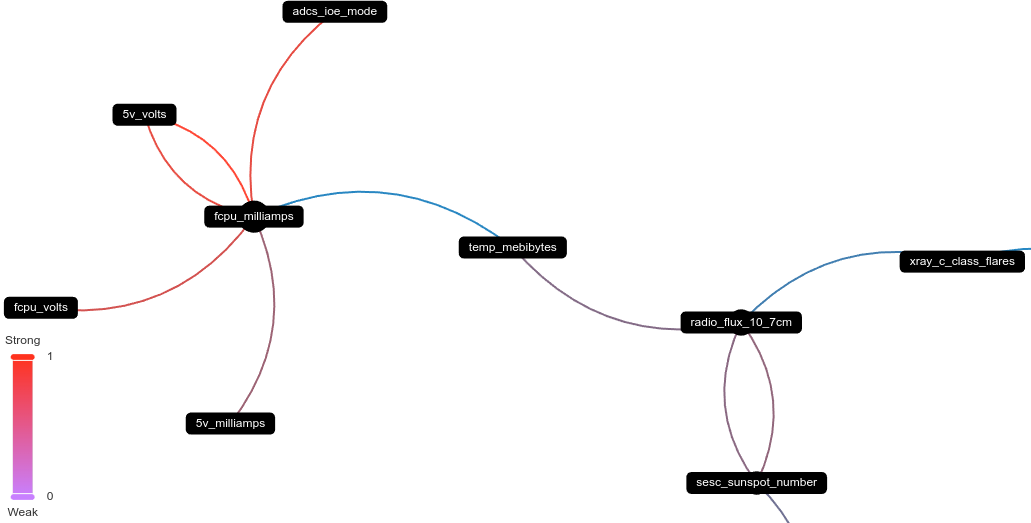
\includegraphics[width=0.95\textwidth]{sat/grifex_dgd.png}
	\caption{Граф кросс-корреляций для основных солнечных и геомагнитных индексов (GRIFEX)}
	\label{fig:grifex_dgd}
\end{figure}

\begin{figure}[H]
	\centering
	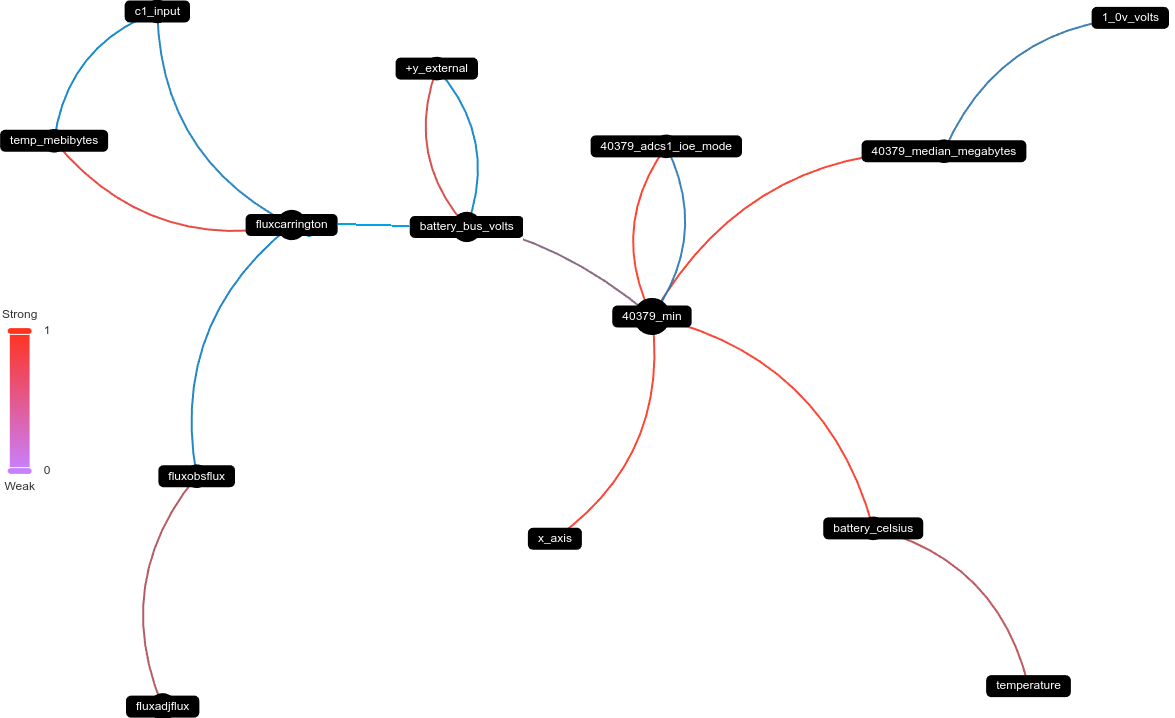
\includegraphics[width=0.95\textwidth]{sat/grifex_flux.png}
	\caption{Граф кросс-корреляций по потокам солнечного радиоизлучения (GRIFEX)}
	\label{fig:grifex_flux}
\end{figure}

\begin{figure}[H]
	\centering
	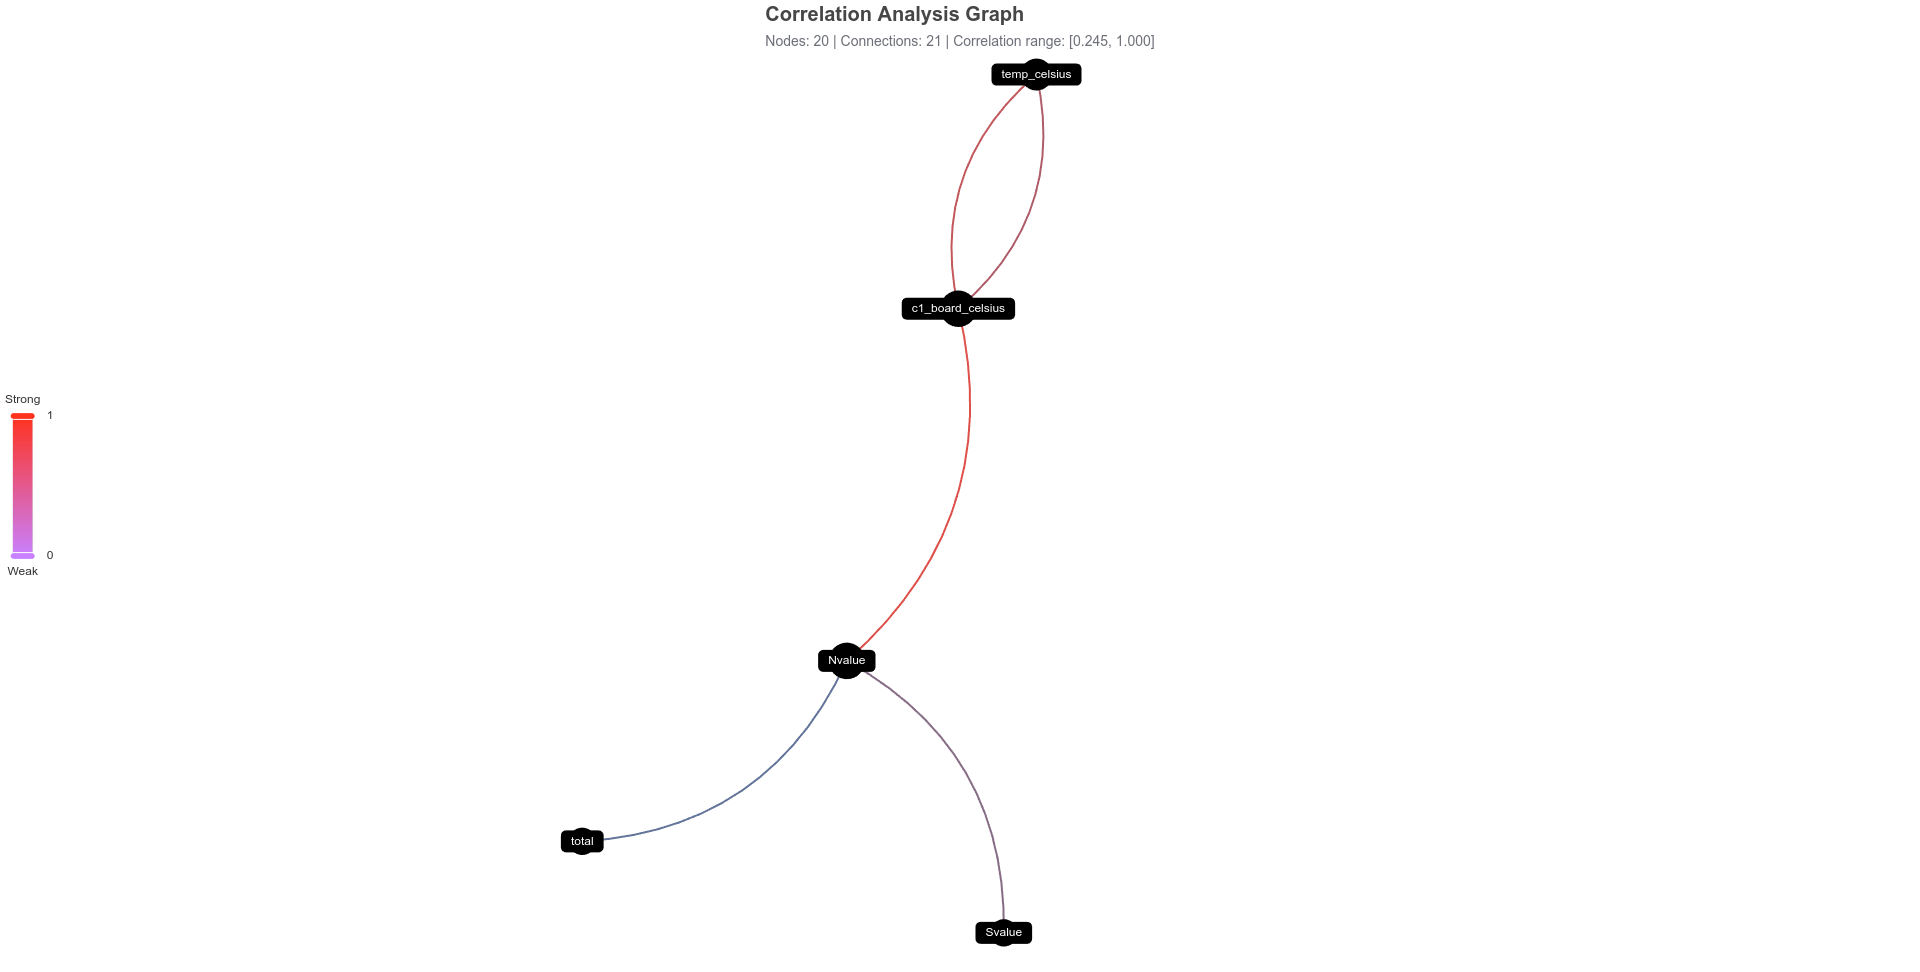
\includegraphics[width=0.95\textwidth]{sat/grifex_hemi.png}
	\caption{Граф кросс-корреляций по параметрам солнечных пятен по полушариям (GRIFEX)}
	\label{fig:grifex_hemi}
\end{figure}

\begin{figure}[H]
	\centering
	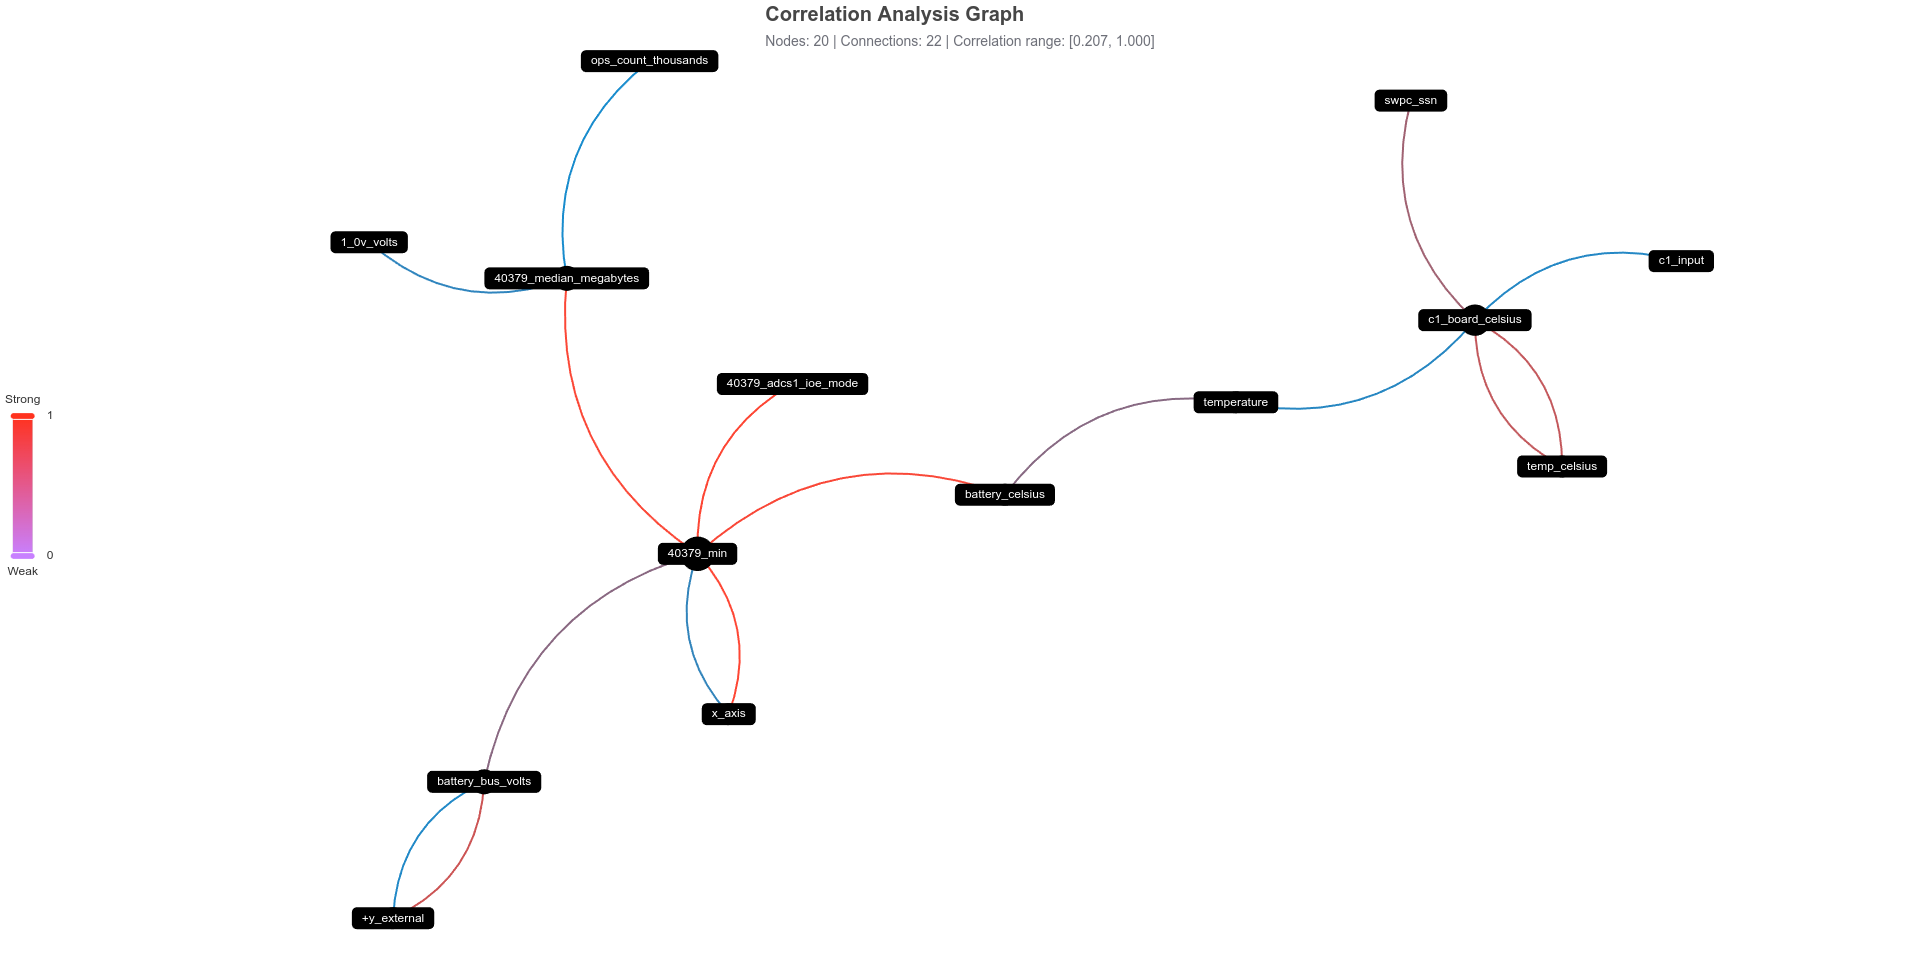
\includegraphics[width=0.95\textwidth]{sat/grifex_ssn.png}
	\caption{Граф кросс-корреляций по числу солнечных пятен (GRIFEX)}
	\label{fig:grifex_ssn}
\end{figure}

\subsection{Структурный анализ и физическая трактовка связей}

Анализируя структуру графов, можно отметить, что наибольшая плотность и сила связей наблюдается между однородными параметрами солнечной активности, такими как среднемесячное число солнечных пятен (\texttt{ssn}), сглаженное число пятен (\texttt{smoothed\_ssn}), а также различные версии наблюдаемых и сглаженных данных по числу пятен (\texttt{observed\_swpc\_ssn}, \texttt{smoothed\_swpc\_ssn}). Это объясняется тем, что все перечисленные параметры отражают одну и ту же физическую сущность - магнитную активность на поверхности Солнца, проявляющуюся в виде пятен, и различаются лишь методикой усреднения и источником данных~\cite{sidc_manual}.

Потоки радиоизлучения (\texttt{f10.7}, \texttt{fluxobsflux}, \texttt{fluxadjflux}, \texttt{fluxursi}) также образуют тесно связанный кластер. Данные параметры измеряются на длине волны 10,7 см и служат стандартом для оценки уровня ультрафиолетового и рентгеновского излучения Солнца, оказывающего непосредственное влияние на ионосферу и, как следствие, на работу радиосистем спутника~\cite{f107_standard}. Сильные корреляции внутри этого кластера подтверждают физическую однородность процессов генерации радиоизлучения на Солнце.

В отличие от солнечных параметров, геомагнитные индексы (\texttt{Fredericksburg A}, \texttt{Fredericksburg K 0-3}, \texttt{K 3-6}, \texttt{K 6-9}) демонстрируют более слабые и разреженные связи с солнечными показателями. Это связано с тем, что геомагнитная активность - результат сложного взаимодействия солнечного ветра и магнитосферы Земли, где задержки и нелинейные эффекты существенно ослабляют прямую корреляцию~\cite{geomag_handbook}. Тем не менее, при анализе временных рядов можно наблюдать, что периоды высокой солнечной активности (рост числа пятен и потока F10.7) приводят к увеличению числа магнитных бурь и, как следствие, к росту значений геомагнитных индексов.


Особый интерес представляет влияние солнечной активности на технические параметры спутника GRIFEX. В отличие от большинства спутников класса CubeSat, GRIFEX построен с применением инновационных архитектурных и технологических решений, ориентированных на работу в условиях повышенного радиационного фона и экстремальных температурных колебаний. Ключевой особенностью является использование гибридного фокального модуля (FPA), в котором кремниевые SiPIN-диоды, произведённые Raytheon Vision Systems, интегрированы с современной БИС-схемой (ROIC) с аналогово-цифровыми преобразователями в каждом пикселе~\cite{norton2012spaceborne, eoportal_grifex}. Это решение обеспечивает не только высокую помехоустойчивость, но и устойчивость к радиационным воздействиям, что нетипично для стандартных CubeSat, традиционно использующих коммерческие компоненты без специальной защиты.

Вся система управления и обработки данных построена на базе FPGA Xilinx Virtex-5, что позволило реализовать отказоустойчивую архитектуру с минимизацией числа точек отказа и резервированием ключевых функций~\cite{eoportal_grifex}. Для GRIFEX были специально выбраны компоненты с повышенной радиационной стойкостью: это касается как цифровых, так и аналоговых трактов. По данным MXL, в конструкцию включены дополнительные экранирующие элементы, а также реализованы алгоритмы коррекции ошибок памяти и мониторинга питания~\cite{mxl_grifex}.

Такой подход позволил существенно снизить количество сбоев и перезагрузок аппаратуры даже в периоды экстремальных солнечных событий, что подтверждается инженерными телеметрическими данными за весь период эксплуатации~\cite{mxl_grifex}. В частности, при увеличении солнечной активности наблюдается рост выработки энергии солнечными панелями, что приводит к повышению токов и напряжений на бортовых шинах. Это, в свою очередь, способствует поддержанию стабильной работы вычислительных блоков и уменьшению числа аварийных перезапусков. Таким образом, положительное влияние солнечной активности проявляется в увеличении энергетического ресурса спутника, при условии эффективной защиты от радиационных воздействий.

На графах кросс-корреляций это выражается в виде сильных связей между параметрами, характеризующими солнечную активность и электрические показатели (ток, напряжение, температура панелей). В периоды низкой солнечной активности, наоборот, возможно снижение выработки энергии, что увеличивает риск сбоев и требует применения дополнительных мер энергосбережения.

\subsection{Заключение}

Структурный анализ графов кросс-корреляций для спутника GRIFEX позволяет сделать следующие выводы. Во-первых, высокая степень корреляции между однородными солнечными параметрами подтверждает корректность и согласованность используемых методик измерения. Во-вторых, относительно слабая связь между солнечными и геомагнитными индексами обусловлена сложностью процессов передачи солнечного воздействия через магнитосферу Земли. В-третьих, применение радиационно-стойких материалов и архитектурных решений обеспечивает устойчивость аппаратуры к солнечным вспышкам, а увеличение солнечной активности, как правило, приводит к росту энергетических возможностей и снижению числа сбоев.

